\chapter{Supplementary Material for Demystifying Spatiotemporal Scaling Laws of Multimodal Video Embeddings}
\label{app:mglvr}

% ============================================================

This document provides additional results and materials referenced in the main paper.
Table~\ref{mglvr:supp:tab:toc} summarises the correspondence between supplementary sections
and main-paper sections.

\begin{table}[htbp]
\centering
\caption{Section correspondence between the supplementary and the main paper.}
\label{mglvr:supp:tab:toc}
\footnotesize
\begin{tabular}{lll}
\toprule
\textbf{Supp.\ Section} & \textbf{Content} & \textbf{Main Paper} \\
\midrule
\S\ref{mglvr:supp:sec:error}   & Error analysis \& case studies       & \S3.2 \\
\S\ref{mglvr:supp:sec:32f}     & Baseline results at 32 frames        & \S4.2 \\
\S\ref{mglvr:supp:sec:scaling} & Additional scaling analyses          & \S4.3-4.4 \\
\S\ref{mglvr:supp:sec:prompts} & LLM prompts used in the pipeline     & \S3.2 \\
\bottomrule
\end{tabular}
\end{table}

% ============================================================
\section{Error Analysis \& Case Studies}
\label{mglvr:supp:sec:error}
% ============================================================

Section~4 of the main paper describes three key failure modes. The corresponding visual case studies are provided below.

\paragraph{(1) Degradation on Long Continuous Temporal Segments.}
As shown in Figure~\ref{mglvr:supp:fig:error1}, the model's performance degrades on long, continuous events. This is because our model, limited by a fixed-length context window (e.g., 16 frames), processes videos in short, independent clips during inference. This segmentation prevents it from capturing the full temporal scope of events that span across multiple clips.

\begin{figure}[htbp]
  \centering
  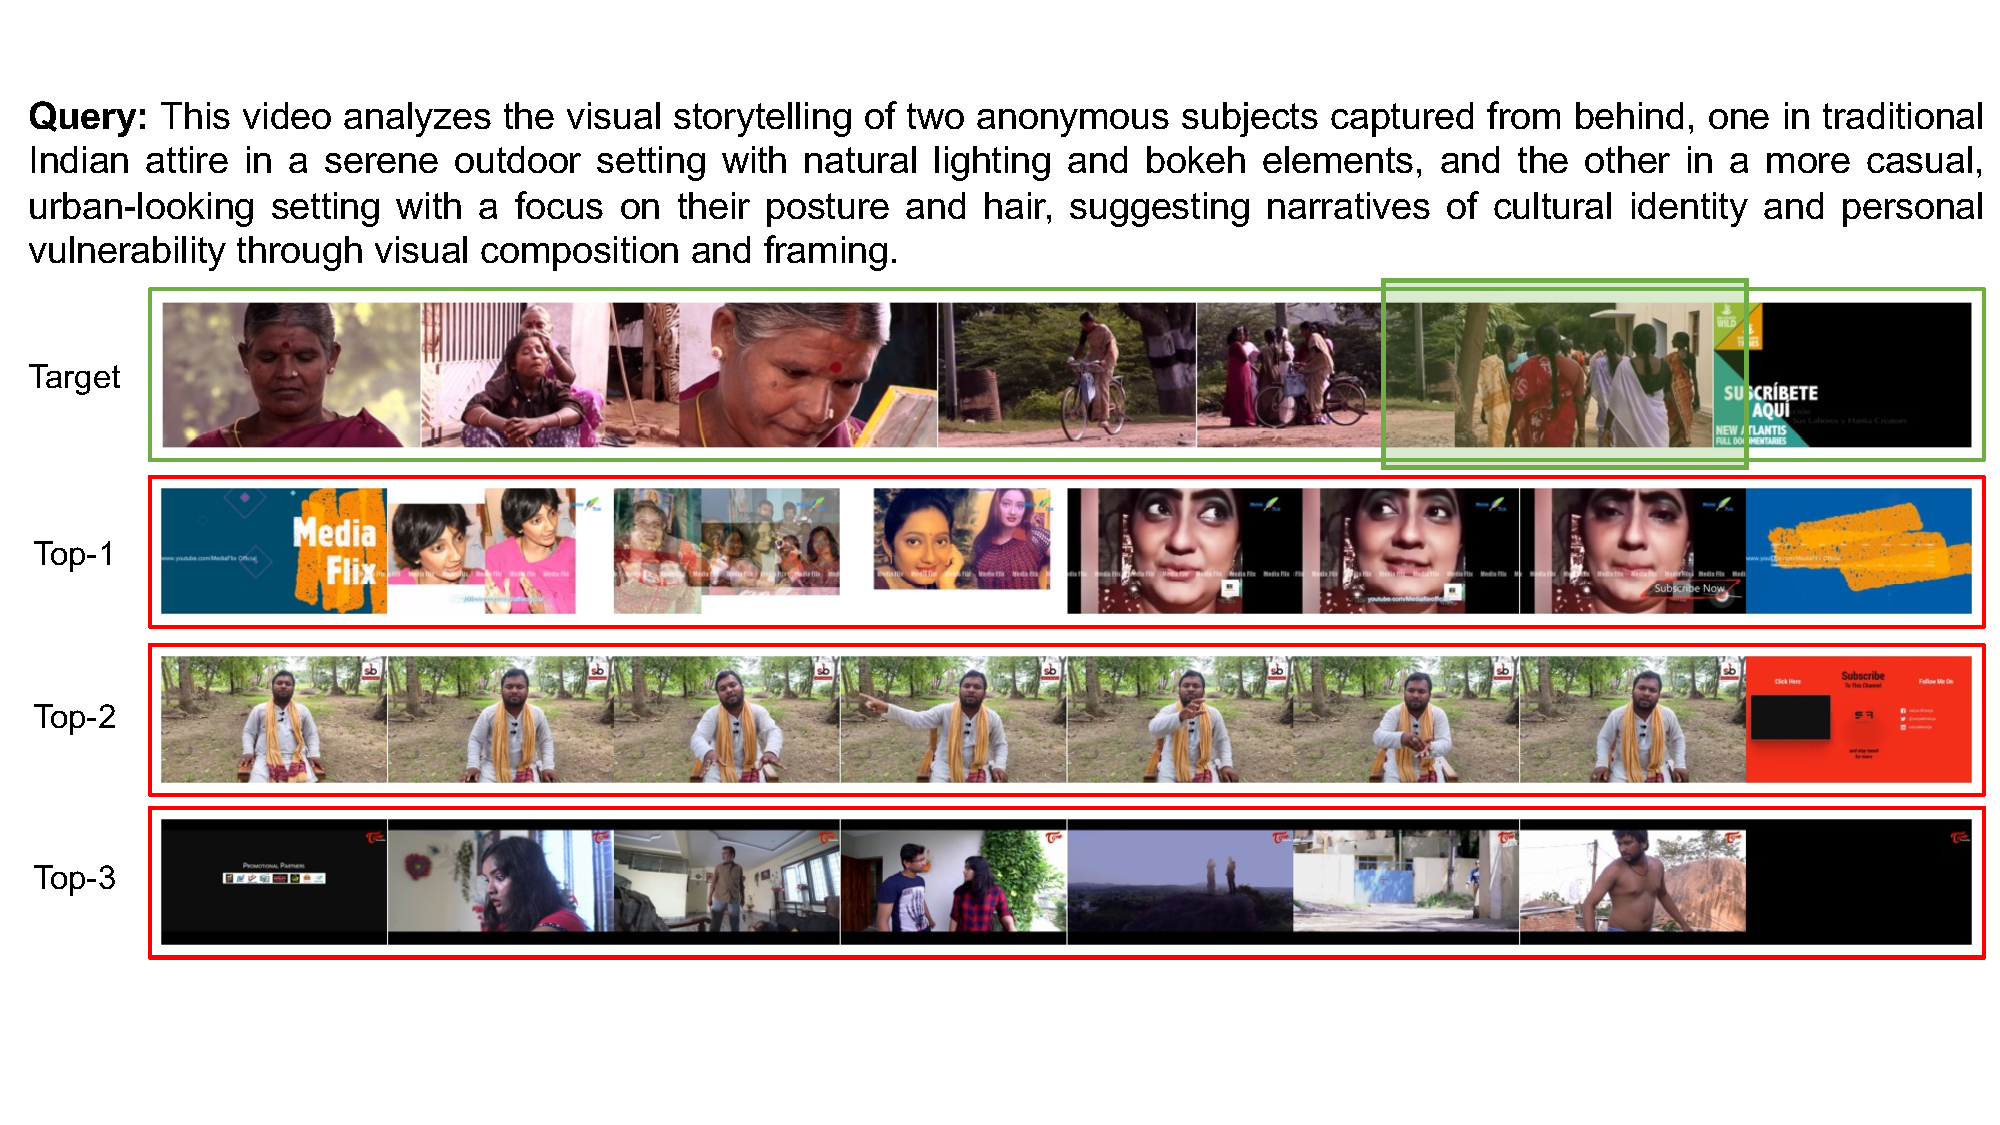
\includegraphics[width=\linewidth]{figures/mglvr/error-analysis/lvr-error-analysis-1.pdf}
  \caption{Example of Error Type 1: \textit{Degradation on Long Continuous Temporal Segments}.}
  \label{mglvr:supp:fig:error1}
\end{figure}

\paragraph{(2) Failure in Fine-Grained Temporal Retrieval.}
As shown in Figure~\ref{mglvr:supp:fig:error2}, this failure occurs when the target event is a brief scene in the background, reflecting difficulties similar to ``needle-in-a-haystack'' scenarios in video retrieval.

\begin{figure}[htbp]
  \centering
  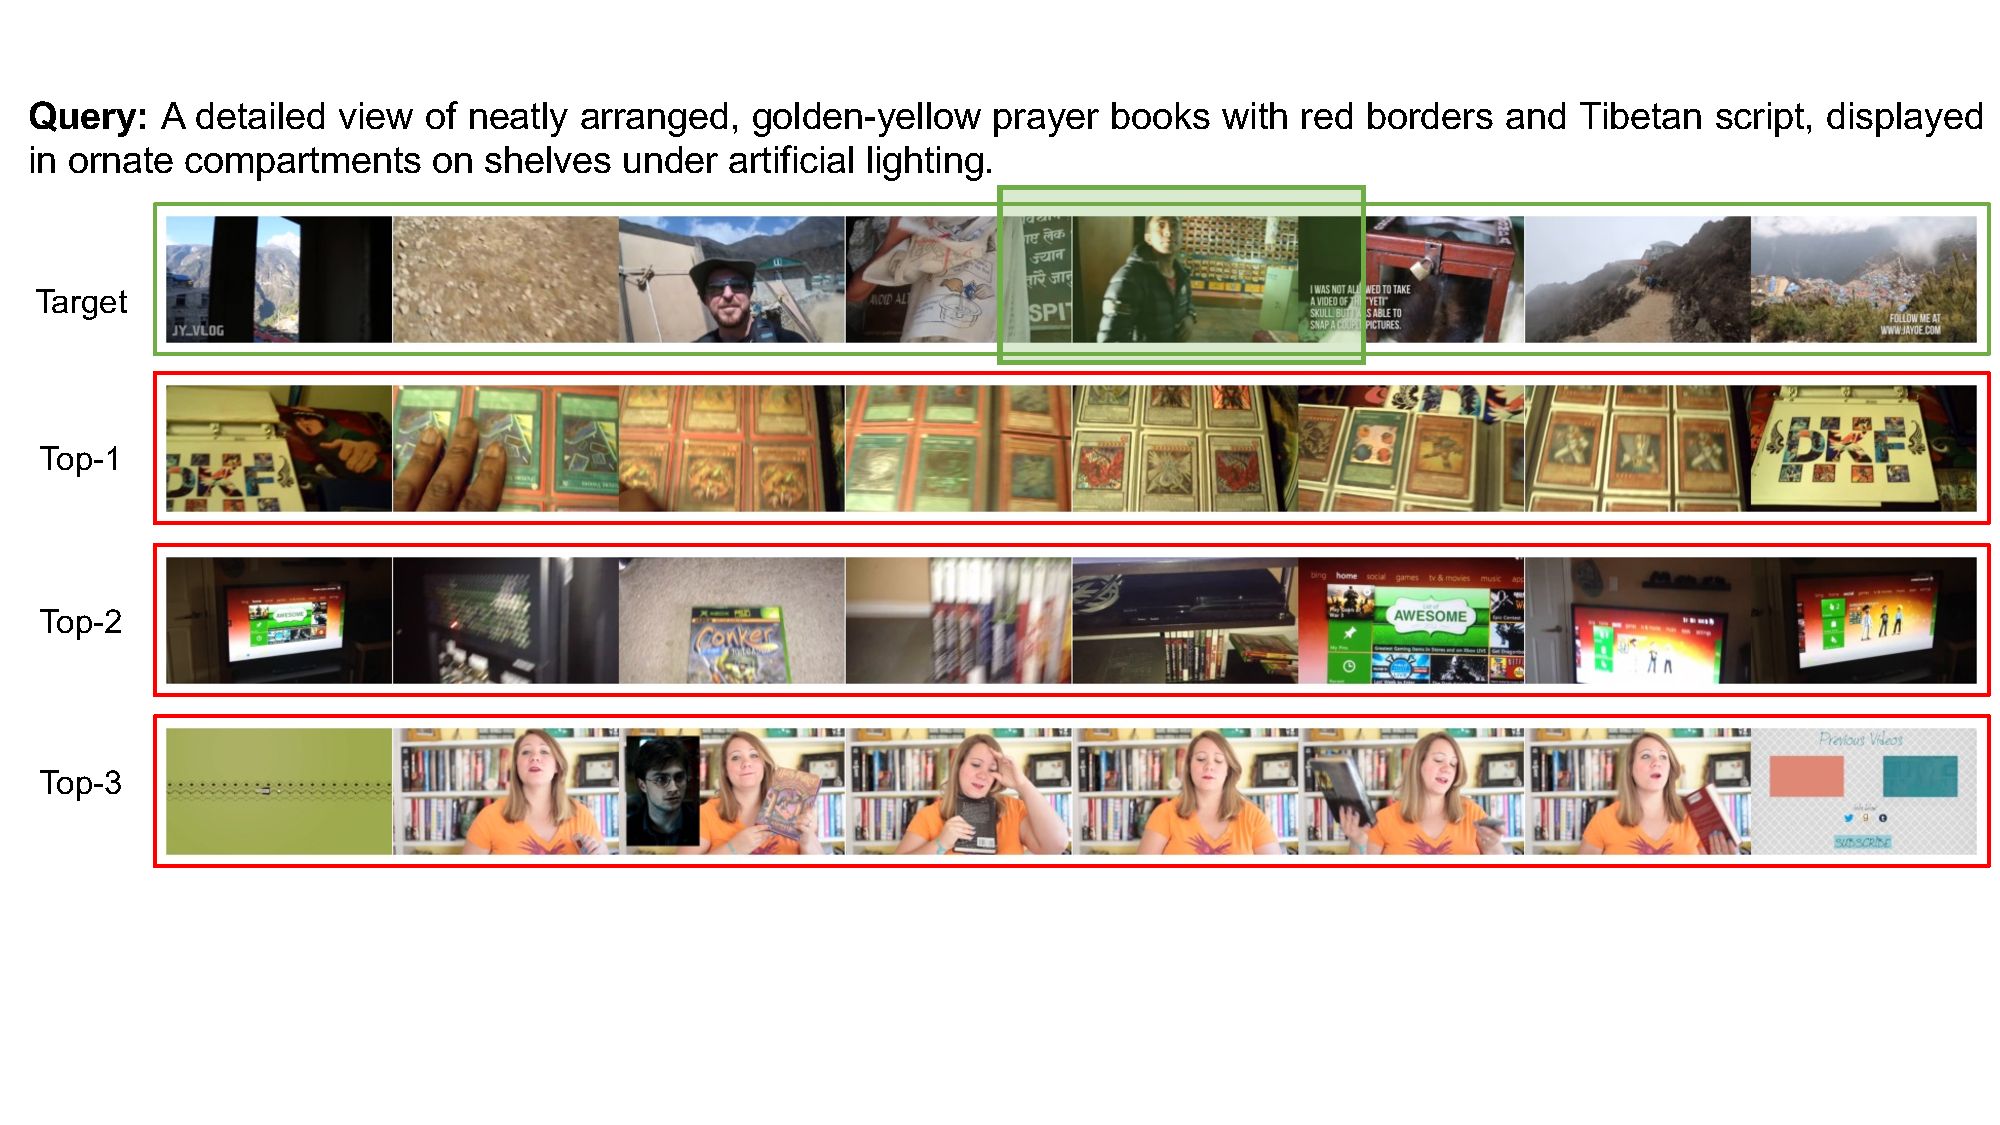
\includegraphics[width=\linewidth]{figures/mglvr/error-analysis/lvr-error-analysis-2.pdf}
  \caption{Example of Error Type 2: \textit{Failure in Fine-Grained Temporal Retrieval}.}
  \label{mglvr:supp:fig:error2}
\end{figure}

\paragraph{(3) Incomplete Satisfaction of Semantic Constraints.}
As shown in Figure~\ref{mglvr:supp:fig:error3}, the model sometimes fails to meet all query conditions. For instance, the top-1 retrieved video satisfies the ``speaker'' requirement but fails to match the ``blue background'' constraint. Similarly, the top-3 retrieved video satisfies most constraints but misses the ``speaker in a patterned shirt'' condition.

\begin{figure}[htbp]
  \centering
  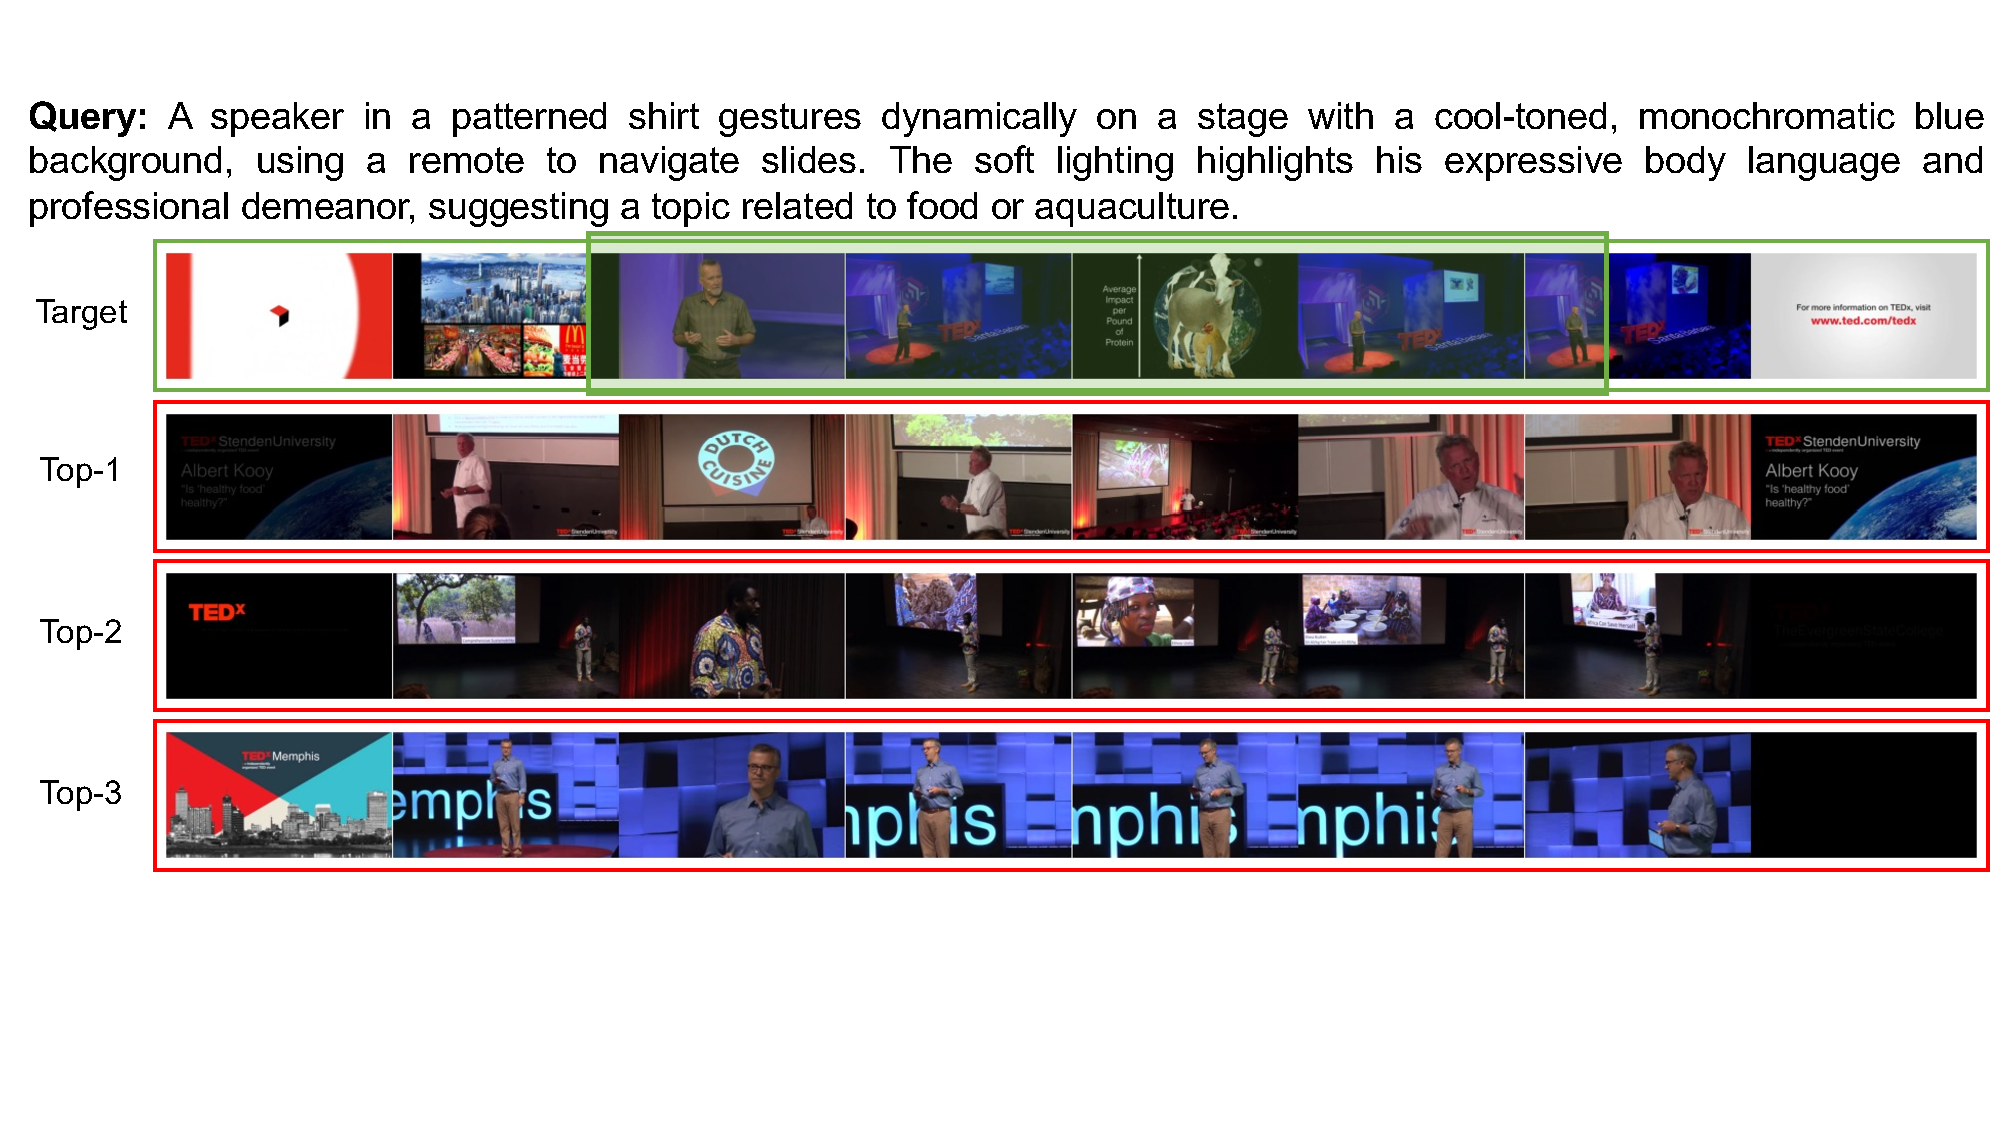
\includegraphics[width=\linewidth]{figures/mglvr/error-analysis/lvr-error-analysis-3.pdf}
  \caption{Example of Error Type 3: \textit{Incomplete Satisfaction of Semantic Constraints}.}
  \label{mglvr:supp:fig:error3}
\end{figure}

% ============================================================
\section{Baseline Results at 32 Frames}
\label{mglvr:supp:sec:32f}
% ============================================================

The main paper (\S3.2) notes that ``results at 32 frames are provided in the supplementary material.'' Table~\ref{mglvr:supp:tab:32f} fills this gap, complementing Table~1 (8\,F) and Table~2 (128\,F) of the main paper.

\begin{table}[htbp]
\centering
\caption{Multi-granularity retrieval performance of all baselines at \textbf{32 uniformly sampled frames} per video. \textbf{Bold} and \underline{underline} indicate the best and second-best results within each model group, respectively.}
\label{mglvr:supp:tab:32f}
\footnotesize
\begin{tabular}{@{}l|*{8}{c}@{}}
\toprule
Model & \multicolumn{2}{c|}{Overall} & \multicolumn{2}{c|}{FN} & \multicolumn{2}{c|}{MD} & \multicolumn{2}{c}{CR} \\
      & R@1 & MRR & R@1 & MRR & R@1 & MRR & R@1 & MRR \\
\midrule
InternVideo2-1B  & 0.1948 & 0.2653 & 0.0463 & 0.0890 & 0.2641 & 0.3611 & 0.5610 & 0.6512 \\
InternVideo2-6B  & 0.2815 & 0.3674 & 0.0963 & 0.1620 & 0.3940 & 0.5022 & \underline{0.6429} & \underline{0.7305} \\
CLIP4Clip        & \underline{0.3087} & \underline{0.3955} & \underline{0.1220} & \underline{0.1924} & \underline{0.4302} & \underline{0.5360} & \underline{0.6429} & 0.7286 \\
LanguageBind     & \textbf{0.4622} & \textbf{0.5445} & \textbf{0.2284} & \textbf{0.3153} & \textbf{0.6374} & \textbf{0.7211} & \textbf{0.7961} & \textbf{0.8538} \\
\midrule
GME-2B           & 0.3407 & 0.4277 & 0.1445 & 0.2183 & 0.4691 & 0.5741 & 0.6892 & 0.7653 \\
Unite-2B         & 0.3672 & 0.4528 & 0.1598 & 0.2352 & 0.5123 & 0.6129 & 0.7008 & 0.7744 \\
Ops-MM-2B        & 0.3832 & 0.4662 & 0.1664 & 0.2412 & 0.5355 & 0.6312 & 0.7302 & 0.8007 \\
VLM2Vec-V2       & 0.4002 & 0.4814 & 0.1721 & 0.2446 & 0.5623 & 0.6574 & 0.7578 & 0.8247 \\
Qwen3-VL-Emb-2B  & \underline{0.4640} & \underline{0.5464} & \underline{0.2091} & \underline{0.2944} & \textbf{0.6562} & \textbf{0.7417} & \underline{0.8237} & \underline{0.8816} \\
GVE-3B           & \textbf{0.4679} & \textbf{0.5487} & \textbf{0.2187} & \textbf{0.3062} & \underline{0.6475} & \underline{0.7302} & \textbf{0.8495} & \textbf{0.8949} \\
\midrule
GME-7B           & 0.3835 & 0.4722 & 0.1560 & 0.2390 & 0.5439 & 0.6435 & 0.7453 & 0.8181 \\
Ops-MM-7B        & 0.4369 & 0.5200 & 0.2085 & 0.2925 & 0.5985 & 0.6879 & 0.7979 & 0.8541 \\
UniME-V2         & 0.4381 & 0.5206 & 0.1876 & 0.2730 & 0.6183 & 0.7054 & 0.8228 & 0.8766 \\
Unite-7B         & 0.4600 & 0.5434 & 0.2138 & 0.3010 & 0.6371 & 0.7269 & 0.8388 & 0.8830 \\
RzenEmbed        & 0.4751 & 0.5546 & 0.2072 & 0.2934 & 0.6729 & 0.7554 & 0.8682 & 0.9089 \\
GVE-7B           & \underline{0.5028} & \underline{0.5833} & \underline{0.2505} & \underline{0.3415} & \underline{0.6873} & \underline{0.7683} & \underline{0.8789} & \underline{0.9144} \\
Qwen3-VL-Emb-8B  & \textbf{0.5290} & \textbf{0.6017} & \textbf{0.2641} & \textbf{0.3497} & \textbf{0.7301} & \textbf{0.7991} & \textbf{0.8976} & \textbf{0.9301} \\
\bottomrule
\end{tabular}
\end{table}

% ============================================================
\section{Additional Scaling Analyses}
\label{mglvr:supp:sec:scaling}
% ============================================================

% ------- B.1 -------
\subsection{Test-Time Spatial Scaling Across Temporal Densities}
\label{mglvr:supp:sec:spatial_scaling}

The caption of Figure~2 in the main paper (\S3.3) notes that ``sensitivity results under varying temporal densities are provided in the supplementary material.'' Figure~\ref{mglvr:supp:fig:spatial_scaling_1} extends Figure~2 by sweeping over $F \in \{8, 32, 128\}$ frames per video, whereas Figure~2 fixes $F = 32$.

\begin{figure}[htbp]
  \centering
  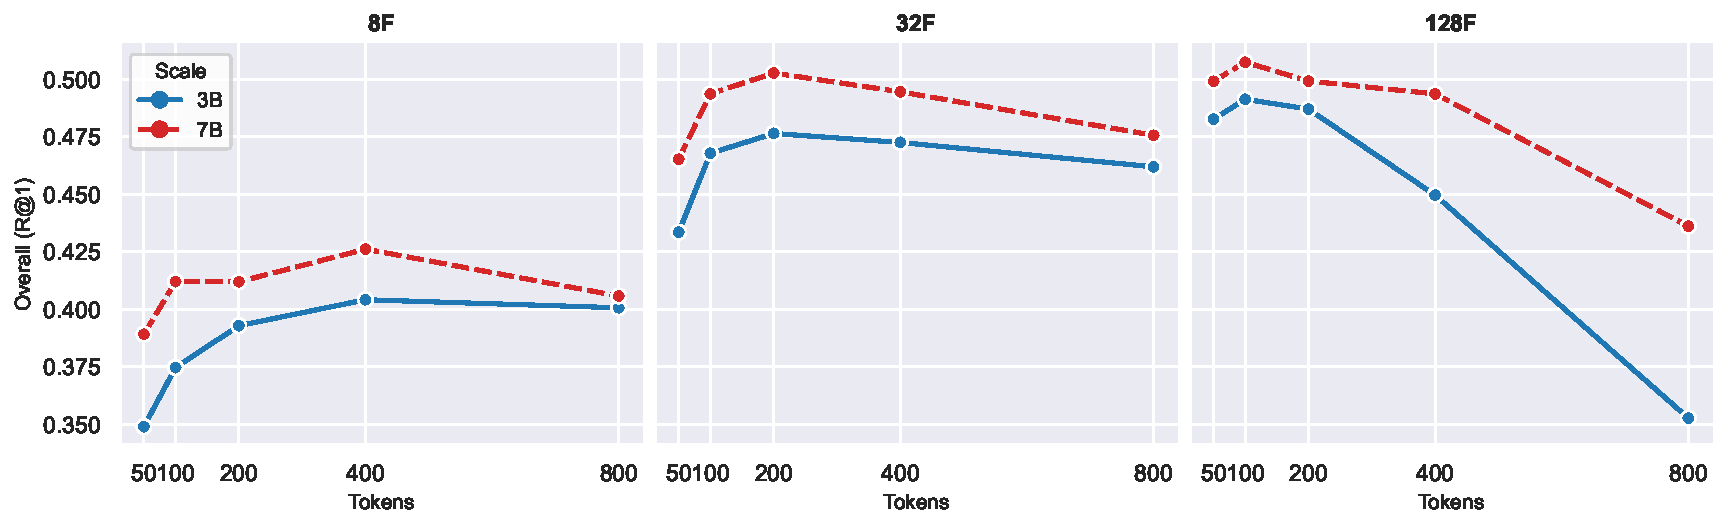
\includegraphics[width=\linewidth]{figures/mglvr/mglvr_testtime_spatial_scaling_1.pdf}
  \caption{Test-time spatial scaling sensitivity of GVE at temporal densities $F \in \{8, 32, 128\}$ frames per video. Each panel fixes $F$ and varies the number of spatial tokens $T$ per frame.}
  \label{mglvr:supp:fig:spatial_scaling_1}
\end{figure}

% ------- B.2 -------
\subsection{Training-Time Spatial Scaling (Evaluated at 8 Test Frames)}
\label{mglvr:supp:sec:train_spatial_8f}

Table~3 of the main paper (\S3.4) reports training-time spatial scaling evaluated at 4 test frames. Table~\ref{mglvr:supp:tab:train_spatial_8f} provides the complementary results at 8 test frames, with $F_{\text{train}}=4$ and $T_{\text{train}} \in \{50, 100, 200, 400\}$.

% The table has 12 columns: cc | cc | cc | cc | cc | cc
% Row format: col1 & col2 & col3 & col4 & col5 & col6 & col7 & col8 & col9 & col10 & col11 & col12 \\
% i.e. exactly 11 ampersands per row.
% For multirow rows: the \multirow cells occupy col1, col3, col4.
% Continuation rows supply col1(train temporal label) & col2(train spatial) & [col3 skipped] & [col4 skipped] & col5..col12

\begin{table}[htbp]
\centering
\caption{Training-time spatial scaling results with fixed temporal density ($F_{\text{train}}=4$), evaluated at \textbf{8 test frames}. Models trained at varying spatial resolutions ($T_{\text{train}} \in \{50, 100, 200, 400\}$) are evaluated across all spatial test configurations. \textbf{Bold} indicates the best result within each group.}
\label{mglvr:supp:tab:train_spatial_8f}
\footnotesize
\begin{tabular}{@{}c@{\hspace{3pt}}c@{\hspace{6pt}}c@{\hspace{3pt}}c@{\hspace{6pt}}*{7}{c@{\hspace{3pt}}}c@{}}
\toprule
\multicolumn{2}{c|}{Training} & \multicolumn{2}{c|}{Testing} & \multicolumn{2}{c|}{Overall} & \multicolumn{2}{c|}{FN} & \multicolumn{2}{c|}{MD} & \multicolumn{2}{c}{CR} \\
Temporal & Spatial & Temporal & Spatial & R@1 & MRR & R@1 & MRR & R@1 & MRR & R@1 & MRR \\
\midrule
\multirow{4}{*}{4F} & 50T  & \multirow{4}{*}{8F} & \multirow{4}{*}{50T}  & 0.2523 & 0.3349 & 0.0941 & 0.1561 & 0.3438 & 0.4461 & 0.5779 & 0.6746 \\
                    & 100T &                      &                       & 0.2567 & 0.3392 & 0.1018 & 0.1620 & 0.3486 & 0.4512 & 0.5672 & 0.6685 \\
                    & 200T &                      &                       & 0.2702 & 0.3529 & 0.1130 & 0.1734 & 0.3607 & 0.4647 & 0.5948 & 0.6928 \\
                    & 400T &                      &                       & \textbf{0.2778} & \textbf{0.3610} & \textbf{0.1137} & \textbf{0.1780} & \textbf{0.3759} & \textbf{0.4773} & \textbf{0.6037} & \textbf{0.6991} \\
\midrule
\multirow{4}{*}{4F} & 50T  & \multirow{4}{*}{8F} & \multirow{4}{*}{100T} & 0.2773 & 0.3598 & 0.1028 & 0.1673 & 0.3793 & 0.4817 & 0.6322 & 0.7169 \\
                    & 100T &                      &                       & 0.2815 & 0.3612 & 0.1065 & 0.1683 & 0.3877 & 0.4851 & 0.6233 & 0.7122 \\
                    & 200T &                      &                       & 0.2907 & 0.3709 & 0.1107 & 0.1752 & 0.3993 & 0.4962 & 0.6447 & 0.7292 \\
                    & 400T &                      &                       & \textbf{0.3041} & \textbf{0.3871} & \textbf{0.1220} & \textbf{0.1897} & \textbf{0.4179} & \textbf{0.5169} & \textbf{0.6474} & \textbf{0.7357} \\
\midrule
\multirow{4}{*}{4F} & 50T  & \multirow{4}{*}{8F} & \multirow{4}{*}{200T} & 0.2889 & 0.3704 & 0.1037 & 0.1691 & 0.4015 & 0.5008 & 0.6500 & 0.7333 \\
                    & 100T &                      &                       & 0.2915 & 0.3721 & 0.1109 & 0.1740 & 0.4000 & 0.4991 & 0.6483 & 0.7341 \\
                    & 200T &                      &                       & 0.2970 & 0.3785 & 0.1105 & 0.1767 & 0.4085 & 0.5076 & 0.6670 & 0.7480 \\
                    & 400T &                      &                       & \textbf{0.3062} & \textbf{0.3883} & \textbf{0.1171} & \textbf{0.1851} & \textbf{0.4242} & \textbf{0.5224} & \textbf{0.6634} & \textbf{0.7453} \\
\midrule
\multirow{4}{*}{4F} & 50T  & \multirow{4}{*}{8F} & \multirow{4}{*}{400T} & 0.2936 & 0.3738 & 0.1041 & 0.1681 & 0.4090 & 0.5076 & 0.6616 & 0.7423 \\
                    & 100T &                      &                       & 0.2977 & 0.3778 & 0.1124 & 0.1754 & 0.4097 & 0.5086 & 0.6607 & 0.7435 \\
                    & 200T &                      &                       & 0.3001 & 0.3800 & 0.1171 & 0.1790 & 0.4090 & 0.5085 & 0.6652 & 0.7488 \\
                    & 400T &                      &                       & \textbf{0.3058} & \textbf{0.3861} & \textbf{0.1203} & \textbf{0.1843} & \textbf{0.4198} & \textbf{0.5175} & \textbf{0.6625} & \textbf{0.7469} \\
\bottomrule
\end{tabular}
\end{table}

% ------- B.3 -------
\subsection{Training-Time Temporal Scaling (Evaluated at 100 Spatial Tokens)}
\label{mglvr:supp:sec:train_temporal_100t}

Table~4 of the main paper (\S3.4) reports training-time temporal scaling evaluated at $T_{\text{test}}=50$ spatial tokens. Table~\ref{mglvr:supp:tab:train_temporal_100t} provides the complementary results at $T_{\text{test}}=100$, with $T_{\text{train}}=50$ and $F_{\text{train}} \in \{4, 8, 16, 32\}$.

\begin{table}[htbp]
\centering
\caption{Training-time temporal scaling results with fixed spatial density ($T_{\text{train}}=50$ tokens per frame), evaluated at \textbf{100 test spatial tokens}. Models trained at varying frame counts ($F_{\text{train}} \in \{4, 8, 16, 32\}$) are evaluated across six temporal test configurations. \textbf{Bold} indicates the best result within each group.}
\label{mglvr:supp:tab:train_temporal_100t}
\footnotesize
\begin{tabular}{@{}c@{\hspace{3pt}}c@{\hspace{6pt}}c@{\hspace{3pt}}c@{\hspace{6pt}}*{7}{c@{\hspace{3pt}}}c@{}}
\toprule
\multicolumn{2}{c|}{Training} & \multicolumn{2}{c|}{Testing} & \multicolumn{2}{c|}{Overall} & \multicolumn{2}{c|}{FN} & \multicolumn{2}{c|}{MD} & \multicolumn{2}{c}{CR} \\
Temporal & Spatial & Temporal & Spatial & R@1 & MRR & R@1 & MRR & R@1 & MRR & R@1 & MRR \\
\midrule
% Group 1: Test 4F-100T
4F  & \multirow{4}{*}{50T} & \multirow{4}{*}{4F}   & \multirow{4}{*}{100T} & \textbf{0.2426} & \textbf{0.3213} & \textbf{0.0935} & \textbf{0.1498} & \textbf{0.3230} & \textbf{0.4222} & \textbf{0.5708} & \textbf{0.6681} \\
8F  &                      &                       &                       & 0.2395 & 0.3189 & 0.0912 & 0.1490 & 0.3213 & 0.4193 & 0.5592 & 0.6609 \\
16F &                      &                       &                       & 0.2251 & 0.3008 & 0.0861 & 0.1408 & 0.2945 & 0.3891 & 0.5512 & 0.6456 \\
32F &                      &                       &                       & 0.2286 & 0.3031 & 0.0916 & 0.1440 & 0.2970 & 0.3908 & 0.5503 & 0.6459 \\
\midrule
% Group 2: Test 8F-100T
4F  & \multirow{4}{*}{50T} & \multirow{4}{*}{8F}   & \multirow{4}{*}{100T} & 0.3116 & 0.3984 & 0.1232 & 0.1943 & 0.4336 & 0.5367 & 0.6509 & 0.7438 \\
8F  &                      &                       &                       & \textbf{0.3188} & \textbf{0.4027} & \textbf{0.1288} & \textbf{0.1979} & \textbf{0.4384} & \textbf{0.5390} & \textbf{0.6741} & \textbf{0.7582} \\
16F &                      &                       &                       & 0.2982 & 0.3828 & 0.1169 & 0.1846 & 0.4116 & 0.5126 & 0.6394 & 0.7345 \\
32F &                      &                       &                       & 0.3045 & 0.3892 & 0.1258 & 0.1925 & 0.4112 & 0.5151 & 0.6598 & 0.7493 \\
\midrule
% Group 3: Test 16F-100T
4F  & \multirow{4}{*}{50T} & \multirow{4}{*}{16F}  & \multirow{4}{*}{100T} & 0.3549 & 0.4422 & 0.1392 & 0.2160 & 0.4988 & 0.6026 & \textbf{0.7284} & \textbf{0.7986} \\
8F  &                      &                       &                       & 0.3553 & 0.4426 & 0.1400 & 0.2172 & 0.5010 & 0.6035 & 0.7204 & 0.7942 \\
16F &                      &                       &                       & \textbf{0.3582} & \textbf{0.4454} & \textbf{0.1405} & \textbf{0.2176} & \textbf{0.5097} & \textbf{0.6114} & 0.7124 & 0.7882 \\
32F &                      &                       &                       & 0.3266 & 0.4116 & 0.1194 & 0.1896 & 0.4611 & 0.5642 & 0.6990 & 0.7793 \\
\midrule
% Group 4: Test 32F-100T
4F  & \multirow{4}{*}{50T} & \multirow{4}{*}{32F}  & \multirow{4}{*}{100T} & 0.3860 & 0.4736 & 0.1619 & 0.2404 & 0.5432 & 0.6462 & 0.7453 & 0.8138 \\
8F  &                      &                       &                       & 0.3805 & 0.4663 & 0.1594 & 0.2362 & 0.5340 & 0.6345 & 0.7409 & 0.8104 \\
16F &                      &                       &                       & \textbf{0.3905} & \textbf{0.4783} & \textbf{0.1664} & \textbf{0.2465} & 0.5483 & \textbf{0.6496} & \textbf{0.7480} & \textbf{0.8179} \\
32F &                      &                       &                       & 0.3877 & 0.4741 & 0.1636 & 0.2434 & \textbf{0.5495} & 0.6457 & 0.7302 & 0.8078 \\
\midrule
% Group 5: Test 64F-100T
4F  & \multirow{4}{*}{50T} & \multirow{4}{*}{64F}  & \multirow{4}{*}{100T} & 0.4086 & 0.4923 & 0.1728 & 0.2538 & \textbf{0.5799} & \textbf{0.6726} & 0.7649 & 0.8266 \\
8F  &                      &                       &                       & 0.3960 & 0.4809 & 0.1696 & 0.2485 & 0.5560 & 0.6530 & 0.7551 & 0.8199 \\
16F &                      &                       &                       & 0.4108 & 0.4961 & 0.1832 & 0.2627 & 0.5739 & 0.6713 & 0.7631 & 0.8284 \\
32F &                      &                       &                       & \textbf{0.4148} & \textbf{0.4994} & \textbf{0.1885} & \textbf{0.2693} & 0.5739 & 0.6699 & \textbf{0.7765} & \textbf{0.8347} \\
\midrule
% Group 6: Test 128F-100T
4F  & \multirow{4}{*}{50T} & \multirow{4}{*}{128F} & \multirow{4}{*}{100T} & 0.4130 & 0.4970 & 0.1859 & 0.2660 & 0.5794 & 0.6723 & 0.7507 & 0.8186 \\
8F  &                      &                       &                       & 0.4013 & 0.4853 & 0.1764 & 0.2556 & 0.5618 & 0.6569 & 0.7516 & 0.8143 \\
16F &                      &                       &                       & 0.4167 & 0.5015 & 0.1840 & 0.2679 & \textbf{0.5843} & 0.6769 & 0.7738 & 0.8330 \\
32F &                      &                       &                       & \textbf{0.4226} & \textbf{0.5073} & \textbf{0.1951} & \textbf{0.2782} & \textbf{0.5843} & \textbf{0.6782} & \textbf{0.7801} & \textbf{0.8368} \\
\bottomrule
\end{tabular}
\end{table}







% ============================================================
\section{Prompts Used in the Pipeline}
\label{mglvr:supp:sec:prompts}
% ============================================================

Section~2.3 of the main paper (Step~4: Retrieval Query Synthesis) uses two LLM prompts: one for generating retrieval queries from clip-level captions (\S\ref{mglvr:supp:sec:prompt_query}), and one for synthesising a consolidated visual description of each video (\S\ref{mglvr:supp:sec:prompt_caption}). Both prompts were executed with Qwen3-32B.

\subsection{Retrieval Query Synthesis}
\label{mglvr:supp:sec:prompt_query}

This prompt is used in Step~4. It receives the aggregated captions of a retrieval unit together with its granularity $G$ and continuity $C$ values, and produces three natural-language queries of increasing descriptive depth.

\begin{promptbox}{Retrieval Query Synthesis from Captions}
\begin{lstlisting}[style=promptstyle]
## ROLE
You are an expert Search Query Synthesizer. Your primary goal is to read a descriptive video caption and generate three high-quality, divergent search queries that are strictly grounded in the visual information provided.

## CRITICAL RULES & PROCESSING LOGIC

### 1. Core Mandate: Grounded and Diverse Queries
- **Strictly Visual & Factual**: All generated queries, regardless of their complexity, MUST be derived solely from the visual information described in the "Raw Caption". Do not invent details not present (e.g., specific brand names unless visible, people's names unless specified as visual text). Explicitly ignore any mention of audio, speech, voice-overs, sound effects, or metadata. Queries must be declarative sentences, not questions or commands.
- **Three Distinct Perspectives**: For each valid caption, generate exactly three queries. These queries must be genuinely different, reflecting diverse user intents and levels of detail.
  - **Query 1 (Librarian/Factual)**: A concise, objective summary of the core visual elements. Length: 20-50 words.
  - **Query 2 (Everyday User/Descriptive)**: A more narrative and descriptive query, using richer vocabulary to describe the scene, actions, and atmosphere. Length: 30-100 words.
  - **Query 3 (Researcher/Analytical)**: A detailed, analytical query that examines visual composition, spatial-temporal details, potential technical aspects, or the narrative storytelling of the scene. Length: 70-200 words.

### 2. Content Quality Filter: Identify and Discard Invalid Inputs
- Before generating queries, you MUST first assess the "Raw Caption" against the following filters. If a caption falls into any of these categories, you MUST return an empty list `[]` for "refined_queries".
- **A clip is considered INVALID if its caption describes:**
  1.  **No Visual Content**: An entirely blank, black, white, or single-color screen with no other discernible objects, text, or shapes.
  2.  **Irretrievably Low Quality**: Content that is explicitly stated to be too blurry, corrupted, pixelated, or overexposed to identify any subjects, objects, or actions.
  3.  **Purely Abstract/Non-Representational**: Content consisting only of abstract patterns, fractals, kaleidoscope effects, or color fields without any concrete, recognizable subjects. (e.g., "a swirling vortex of psychedelic colors").
  4.  **Extremely Low Information Density**: A single, simple, static, or looping scene with minimal change over a long duration, making the generation of three diverse, meaningful queries impossible. (e.g., "a 10-minute video of a spinning fan" or "a static image of a single apple on a table").
  5.  **Dense Text/Code as Primary Content**: Screen recordings that primarily show large, scrolling blocks of code, documents, or dense text where the main subject is the textual information itself, not a visual narrative or action. (This does not apply to simple title cards or logos).
  6.  **Refusals or Error Messages**: The caption is an apology, a refusal to describe (e.g., "I'm sorry, I cannot describe..."), or an error message.

### 3. Special Handling for Minimalist Content
- If the caption describes a very simple scene (e.g., a plain background) but **also contains a key visual element** like a logo, a title card, or a single piece of text (e.g., 'LATINO' on a black screen), it is considered **VALID**.
- In such cases, your queries must **focus intently on these minimal elements**. Describe their visual properties (font, color, style, placement) and, for the researcher query, analyze their likely function (e.g., branding, title sequence, call-to-action).

## OUTPUT FORMAT
You MUST return ONLY a single, strict JSON object. No explanations or conversational text. The required format is:
{"refined_queries": ["Librarian query text", "Everyday user query text", "Researcher query text"]}

- If the input is deemed invalid based on the "Content Quality Filter", the output MUST be:
{"refined_queries": []}

**Metadata**: Granularity={granularity}, Continuity={continuity}
**Raw Caption**: {caption}

**JSON Output**:
\end{lstlisting}
\end{promptbox}

\subsection{Clip Caption Merging}
\label{mglvr:supp:sec:prompt_caption}

This prompt produces a consolidated visual-only description of each video from its clip-level captions. The output serves as the semantic proxy for building the Clip Relation Graph ($\mathcal{G}$) in Step~2, and is also used during the refinement pass in Step~4 to filter out queries that reference non-visual content.

\begin{promptbox}{Clip Caption Merging in Groups}
\begin{lstlisting}[style=promptstyle]
## Role & Core Principle
You are a master video summarizer, operating as a **Visual Purist**. Your absolute primary goal is to create a single, flowing paragraph that describes only what a person would see if they watched the video with the sound completely off.

**Your Most Important Rule: Proactive Filtering.**
You MUST critically analyze the input `caption` for each clip and proactively filter out any information that is not strictly visual. **Completely ignore and do not mention**:
-   **Spoken Content**: Dialogue, narration, interviews, or any transcribed speech (e.g., "the narrator explains...", "discusses the importance of...").
-   **Character/Object Names & Backstories**: Proper names of people, places, or things (e.g., "Midas the mouse," "the Napa fires"), unless they are clearly visible as text in the scene (e.g., a brand name on a product).
-   **Abstract Concepts & Inferred Knowledge**: Intentions, emotions, technical jargon (e.g., "'Inverted Single Stroke Four' drum fill"), or specialized knowledge that cannot be seen directly (e.g., "the car's engine is powerful").
-   **Audio Cues**: Descriptions of music, sound effects, or tone of voice.

## Input Analysis & Synthesis Logic
Follow this structured three-step process to generate the summary:

**Step 1: Identify the Core Subject & Setting.**
-   Quickly scan all clip captions to determine the recurring central subject (e.g., a person, an animal, an object) and the primary environment (e.g., a kitchen, a forest, a studio). This forms the foundation of your summary.

**Step 2: Construct the Narrative Flow.**
-   Start your summary by introducing the core subject and setting you identified.
-   Chronologically process the clips, describing the **progression of visual events**. Use temporal cues like "The video begins with...", "As the demonstration progresses...", "Later, the scene shifts to...", and "The video concludes by showing..." to create a coherent narrative.
-   Give more descriptive weight to clips with a higher `temporal_ratio`, as they represent more of the video's runtime.
-   **Crucially**, also integrate unique, visually striking details from shorter clips, especially if they show a distinct action, a close-up of a key object, or a significant change in the scene. This ensures the summary is both representative and rich in detail.

**Step 3: Refine and Polish.**
-   Ensure the final text is a single, well-written paragraph.
-   Read through your summary one last time to confirm it is 100 percent based on visual information and flows logically from beginning to end.

## Handling Inconsistencies & Corner Cases
-   **Conflicting Visuals**: If clips describe conflicting details (e.g., wall color changes from 'purple' to 'beige'), either describe the most dominant/frequently-seen version or briefly acknowledge the change (e.g., "...in a room with walls that appear alternately purple and beige."). **Do not** create an inaccurate hybrid description.
-   **Invalid/Empty Clips**: If a clip's caption is an error message, a refusal, or contains no visual information, ignore it completely.

## Output Specification
-   Your output MUST be ONLY a single, valid JSON object.
-   The JSON object must have two keys: `video_id` (string) and `caption` (string).
-   The `caption` should be a single paragraph, typically between 30 and 200 words.

## Input
Video ID: {video_id}
Clips (clip_id | caption | span | ratio):
{clips}
\\

\#\# Output:
\end{lstlisting}
\end{promptbox}
